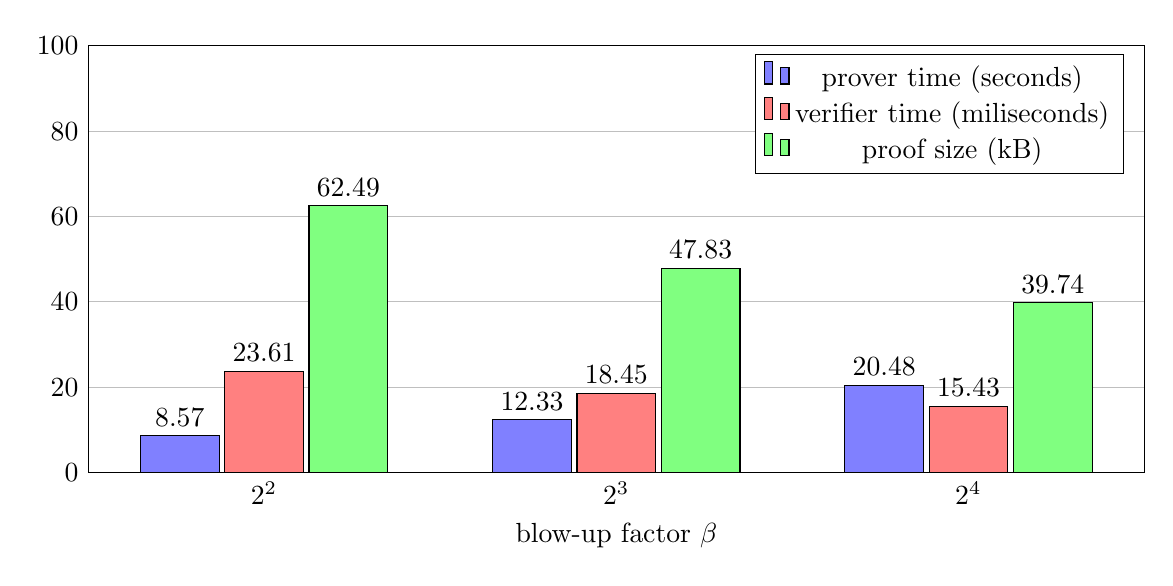
\begin{tikzpicture}
    \centering
    \begin{axis}[
        ybar,
        % title={Benchmarks for preliminary implementation},
        height=7cm, width=15cm,
        bar width=1cm,
        xmode=log, log basis x=2,
        xmin=2.83, xmax=22.63,
        xlabel={blow-up factor $\beta$},
        ymajorgrids,
        ymin=0, ymax=100,
        tickwidth=0pt,
        nodes near coords={
            \pgfmathprintnumber[precision=2]{\pgfplotspointmeta}
        },
    ]
        \addplot [draw, fill=blue!50] coordinates {
            (4,8.57)
            (8,12.33)
            (16,20.48)
        };
        \addplot [draw, fill=red!50] coordinates {
            (4,23.61)
            (8,18.45)
            (16,15.43)
        };
        \addplot [draw, fill=green!50] coordinates {
            (4,62.49)
            (8,47.83)
            (16,39.74)
        };
        \legend{prover time (seconds),verifier time (miliseconds),proof size (kB)}
        % \addplot [draw=blue, xshift=-1cm] plot[smooth] coordinates {
        %     (4,8.57)
        %     (8,12.33)
        %     (16,20.48)
        % };
        % \addplot [draw=red] plot[smooth] coordinates {
        %     (4,23.61)
        %     (8,18.45)
        %     (16,15.43)
        % };
        % \addplot [draw=green, xshift=1cm] plot[smooth] coordinates {
        %     (4,62.49)
        %     (8,47.83)
        %     (16,39.74)
        % };
    \end{axis}
\end{tikzpicture}